\documentclass[border=10pt,margin=5pt,tikz,dvisvgm,rgb,utf8]{standalone}
\usepackage{ctex,xeCJK}  % 中文环境
\setCJKmainfont[BoldFont=Source Han Sans SC]{Source Han Serif SC}
\usepackage{calc,fontawesome,forest,smartdiagram,xcolor}
\usetikzlibrary{animations,arrows,automata,graphs,matrix,positioning,shadows,shapes}

\begin{document}
\renewcommand{\baselinestretch}{0.4}

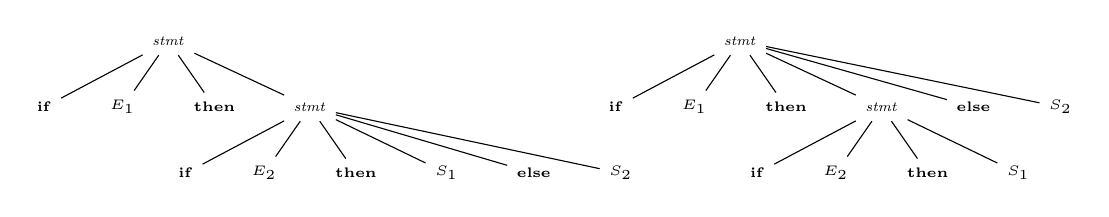
\begin{tikzpicture}
  % A
  \node[](Aif1){\tiny \textbf{if}};
  \node[right=0.5 of Aif1](Ae2){\tiny $E_{2}$};
  \node[right=0.5 of Ae2](Athen1){\tiny \textbf{then}};
  \node[right=0.5 of Athen1](As1){\tiny $S_{1}$};
  \node[right=0.5 of As1](Aelse1){\tiny \textbf{else}};
  \node[right=0.5 of Aelse1](As2){\tiny $S_{2}$};
  \node[above=0.66 of $(Ae2)!0.5!(Athen1)$](Astmt1){\tiny \textit{stmt}};
  \node[left=0.5 of Astmt1](Athen2){\tiny \textbf{then}};
  \node[left=0.5 of Athen2](Ae1){\tiny $E_{1}$};
  \node[left=0.5 of Ae1](Aif2){\tiny \textbf{if}};
  \node[above=0.66 of $(Ae1)!0.5!(Athen2)$](Astmt2){\tiny \textit{stmt}};
  \path[-]
  (Astmt1) edge (Aif1)
  (Astmt1) edge (Ae2)
  (Astmt1) edge (Athen1)
  (Astmt1) edge (As1)
  (Astmt1) edge (Aelse1)
  (Astmt1) edge (As2)
  (Astmt2) edge (Aif2)
  (Astmt2) edge (Ae1)
  (Astmt2) edge (Athen2)
  (Astmt2) edge (Astmt1);

  % B
  \node[right=1.25 of As2](Bif1){\tiny \textbf{if}};
  \node[right=0.5 of Bif1](Be2){\tiny $E_{2}$};
  \node[right=0.5 of Be2](Bthen1){\tiny \textbf{then}};
  \node[right=0.5 of Bthen1](Bs1){\tiny $S_{1}$};
  \node[above=0.66 of $(Be2)!0.5!(Bthen1)$](Bstmt1){\tiny \textit{stmt}};
  \node[left=0.5 of Bstmt1](Bthen2){\tiny \textbf{then}};
  \node[left=0.5 of Bthen2](Be1){\tiny $E_{1}$};
  \node[left=0.5 of Be1](Bif2){\tiny \textbf{if}};
  \node[right=0.5 of Bstmt1](Belse1){\tiny \textbf{else}};
  \node[right=0.5 of Belse1](Bs2){\tiny $S_{2}$};
  \node[above=0.66 of $(Be1)!0.5!(Bthen2)$](Bstmt2){\tiny \textit{stmt}};
  \path[-]
  (Bstmt2) edge (Bif2)
  (Bstmt2) edge (Be1)
  (Bstmt2) edge (Bthen2)
  (Bstmt2) edge (Bstmt1)
  (Bstmt2) edge (Belse1)
  (Bstmt2) edge (Bs2)
  (Bstmt1) edge (Bif1)
  (Bstmt1) edge (Be2)
  (Bstmt1) edge (Bthen1)
  (Bstmt1) edge (Bs1);
\end{tikzpicture}

\end{document}
